\documentclass{standalone}
\usepackage{tikz}

\begin{document}

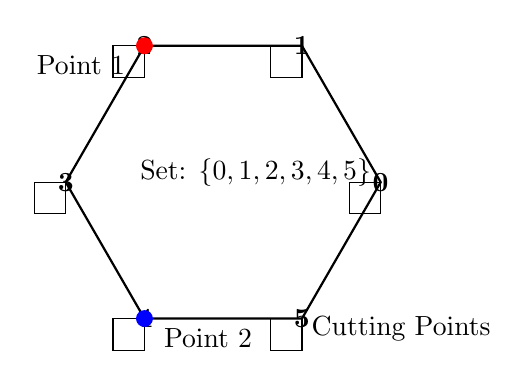
\begin{tikzpicture}[scale=2]
    % Define the positions of the boxes
    \foreach \i in {0,1,2,3,4,5} {
        \node (box\i) at ({cos(60*\i)}, {sin(60*\i)}) {};
        \draw (box\i) rectangle ++(-0.2,-0.2);
        \node at (box\i) {\textbf{\i}};
    }

    % Draw the circle connecting the boxes
    \draw[thick] (box0.center) -- (box1.center) -- (box2.center) -- (box3.center) -- (box4.center) -- (box5.center) -- cycle;

    % Indicate the cutting points
    \filldraw[red] (box2.center) circle (0.05);
    \filldraw[blue] (box4.center) circle (0.05);

    % Add labels for clarity
    \node[left] at (box0.north) {Set: $\{0, 1, 2, 3, 4, 5\}$};
    \node[right] at (box5.south) {Cutting Points};
    \node[below left] at (box2.west) {Point 1};
    \node[below right] at (box4.east) {Point 2};

\end{tikzpicture}

\end{document}